\clearpage
\section{Arduino Quantum Receiver}

\begin{refsection}
	
	\begin{tcolorbox}	
		\begin{tabular}{p{2.75cm} p{0.2cm} p{10.5cm}} 	
			\textbf{Student Name}  		&:&  Jo\~ao Fraz\~ao (2019/09/02 - )\\
			&:&  Eduardo Fernandes (2019/06/15 - 2019/09/14)\\
			\textbf{Goal}          &:& Implement the QKD reception module in an Arduino (Coincidence Detector, QBER, Source and Sink blocks).\\
			\textbf{Directory}              &:& sdf/arduino\_quantum\_rx
		\end{tabular}
	\end{tcolorbox}
	
	
	\subsection{Project Definition}
	
		The purpose of this project is to implement the QKD reception module of a quantum communication system, into an arduino board. To achieve this goal we need to know what the arduino is going to receive and what's going to output.
		There are two classical signals, that are going to be read by two single photon detectors. These signals are the clock, which are going to synchronize the quantum detectors. The next block of implementation in the arduino is the coincidence detector and it contains the signals provenient from the single-photon dectectors which can be 0 or 1. In addition, this block outputs a signal containing a state corresponding to the input values:3 if no-click has been detected, 2 if both detectors clicked, 1 if bit one was measured, and finally, 0 if bit zero was measured. The last block that needs to be implemented is the IPtunnel which corresponds to the communication protocol. This block is responsible for the trasnmission of the coincidence detector output in the arduino (client side) to a pc (server side) through a ehthernet connection.
	
	\begin{figure}[H]
		\centering
		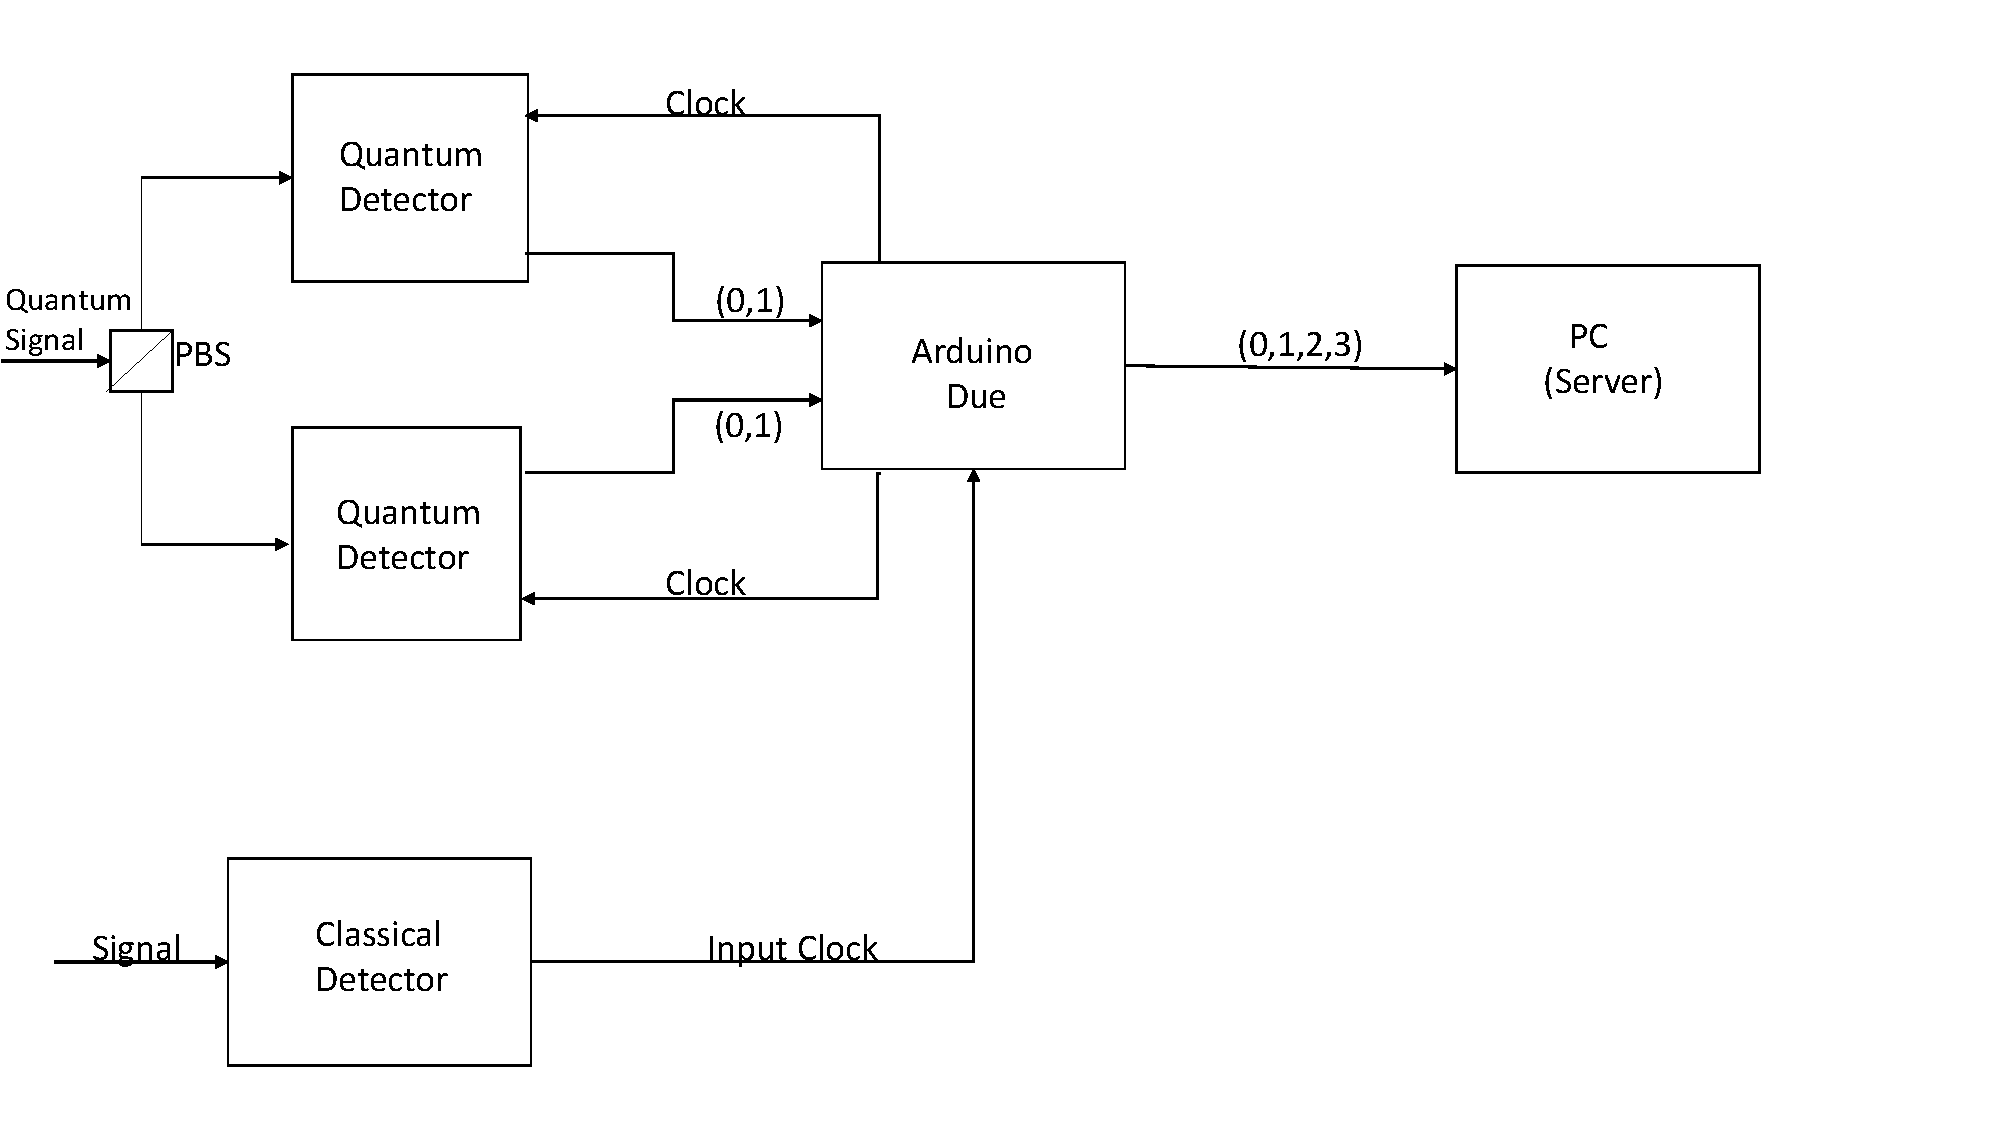
\includegraphics[width=1\linewidth]{./sdf/arduino_quantum_rx/figures/DiagramaGeral.pdf}
		\caption{General block diagram of QKD a quantum receiver module.}
		\label{fig:arduino}
	\end{figure}


		
	\subsection{Emulation in NetXPTO Simulator}
	
	For the emulation in the NetXPTO Simulator, we have to run two seperate codes. The first one corresponds to the client side of the simulation which can be found in the arduino\_quantum\_rx\_netxpto project. The second one is the server side and can be found in the ip\_tunnel\_ms\_windows - Server project. In order to have the emulation working it is needed both programs running simultaneously.
	
	\begin{figure}[H]
		\centering
		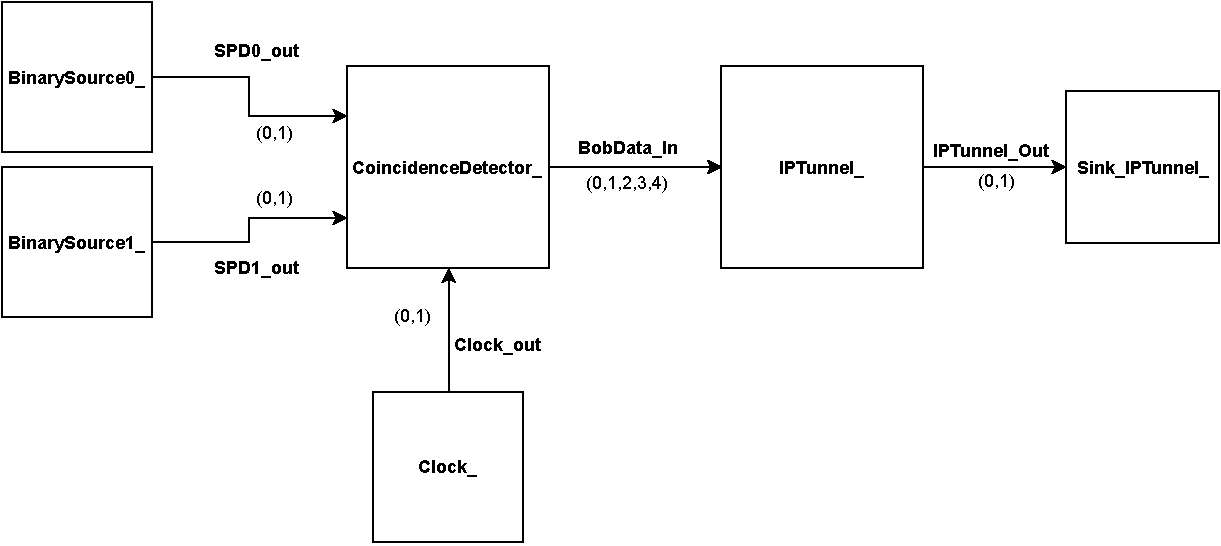
\includegraphics[width=0.9\linewidth]{./sdf/arduino_quantum_rx/figures/NetXPTO_implementation.pdf}
		\caption{Block diagram of a quantum receiver system emulated in NetXPTO (Client side).}
		\label{fig:netxpto}
	\end{figure}

	\begin{figure}[H]
		\centering
		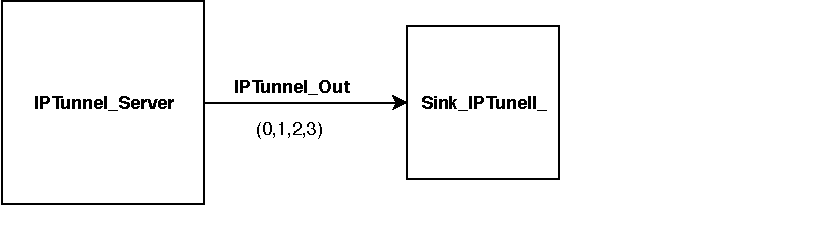
\includegraphics[width=0.9\linewidth]{./sdf/arduino_quantum_rx/figures/NetXPTO_2.pdf}
		\caption{Block diagram of a quantum receiver system emulated in NetXPTO (Server side).}
		\label{fig:netxpto}
	\end{figure}
	
	For the client side in NetXPTO Simulator we have to implement the following 5 modules . The first two are the BinarySource0\_ and the BinarySource1\_ which emulates the received signals provenient from the single-photon detectors 0 and 1, respectively, and are synchronized by the Clock\_ block. These signals are the inputs of the CoincidenceDetector\_ block, that in its turn, outputs a real signal that has five possible values: 4 correspondes to the null values of the buffer when the clock is in the low state, 3 if no-click has been detected, 2 if both detectors clicked, 1 if bit one was measured, and finally, 0 if bit zero was measured. Finally, we have the IPTunnel\_Client\_ block that is responsible for the comumunications between the client and the PC server. It uses a TCP/IP protocol to communicate with the IPTunnel\_Server , which takes the output of the signal from the CoincidenceDetector\_ block and sends it to the server implemented in a PC, where the QBER estimations are performed. \\ \\

	
	The following input parameters were defined for the blocks listed in figure \ref{fig:netxpto}:
	
	\begin{itemize}
		\item BinarySource0\_:
		\begin{itemize}
			\item setMode(BinarySourceMode::DeterministicCyclic)
			\item setBitStream("1")
		\end{itemize}
	
		\item BinarySource1\_:
		\begin{itemize}
			\item setMode(BinarySourceMode::DeterministicCyclic)
			\item setBitStream("0")
		\end{itemize}
		
		\item Clock\_:
		\begin{itemize}
			\item setClockPeriod(1e-6)
			\item setSamplingPeriod(1e-7)
		\end{itemize}
		
		\item CoincidenceDetector\_;
		
		\item IPTunnel\_;
		

			
		\end{itemize}
%	\end{itemize}


\vspace{15px}


\textbf{Signal Results:}

\begin{itemize}
	
	\item SPD0\_out:
	\begin{figure}[H]
		\centering
		\includegraphics[width=1\linewidth]{./sdf/arduino_quantum_rx/figures/spd0.png}
		\caption{Signal generated from BinarySource0.}
		\label{fig:arduino}
	\end{figure}

	\vspace{50px}
	\item SPD1\_out:
	\begin{figure}[H]
		\centering
		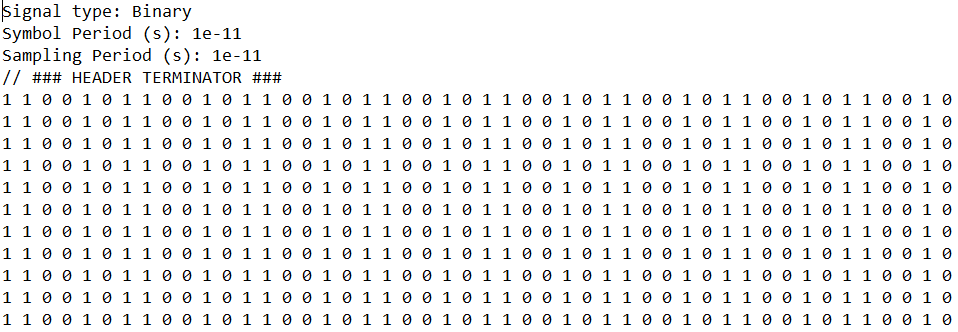
\includegraphics[width=1\linewidth]{./sdf/arduino_quantum_rx/figures/spd1.png}
		\caption{Signal generated from BinarySource1.}
		\label{fig:arduino}
	\end{figure}

	
	\item Clock\_out:
	\begin{figure}[H]
		\centering
		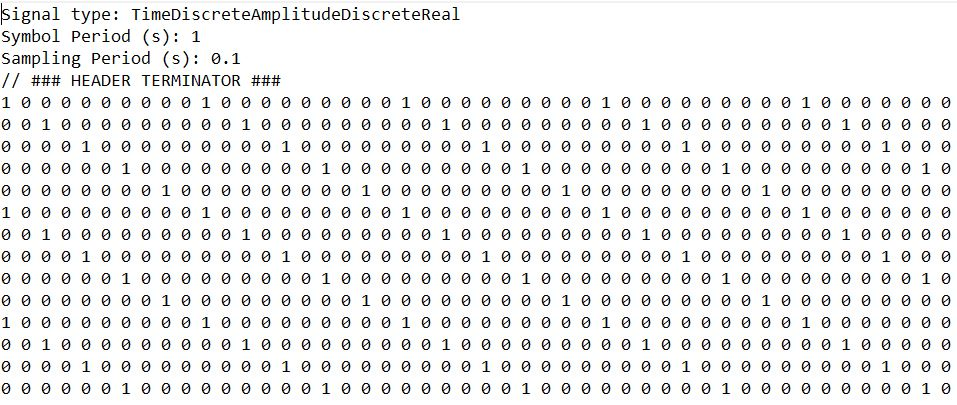
\includegraphics[width=1.1\linewidth]{./sdf/arduino_quantum_rx/figures/Clock.JPG}
		\caption{Signal generated from Clock.}
		\label{fig:arduino}
	\end{figure}
	\clearpage
	
	\item BobData\_In;
	\begin{figure}[H]
		\centering
		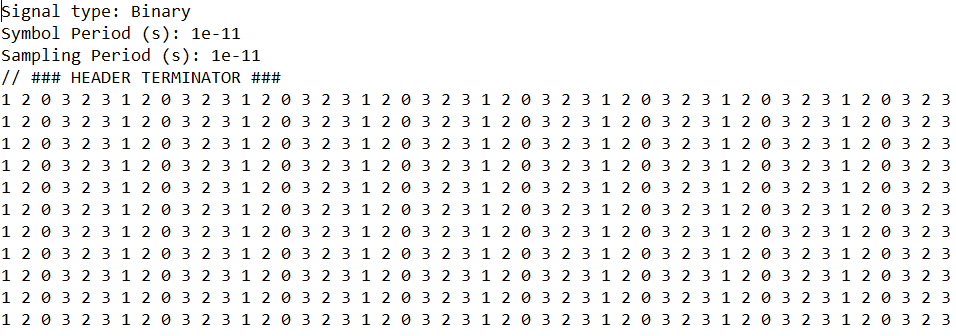
\includegraphics[width=1.1\linewidth]{./sdf/arduino_quantum_rx/figures/Bobdatain.PNG}
		\caption{Signal generated from CoincidenceDetector.}
		\label{fig:arduino}
	\end{figure}

		\item IPTunnel\_Out;
	\begin{figure}[H]
		\centering
		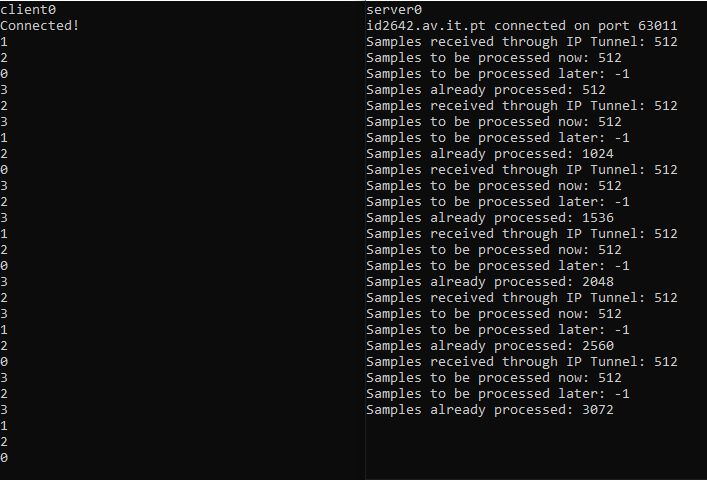
\includegraphics[width=1\linewidth]{./sdf/arduino_quantum_rx/figures/Iptunnel.PNG}
		\caption{Signal the client is sending through the IPTunnel block and what the server is receiving.}
		\label{fig:arduino}
	\end{figure}

\end{itemize}
	
	
	
	
	
	\subsection{Simulation Analysis - Arduino Implementation}
	
	In order to utilize the same project running over NetXPTO simulator using Arduino technology some changes in the source code had to be made once this technology uses C/C++ language features while relying on special rules of code structuring. Acoording to Arduino official manufactures this language is merely a set of C/C++ functions that can be called from your code. Your sketch undergoes minor changes (e.g. automatic generation of function prototypes) and then is passed directly to a C/C++ compiler (avr-g++). \par However, there's currently no support for libstdc++, the standard support library needed for a complete C++ implementation. This imposes a number of restrictions on the C++ programs that can be compiled. Among them are:
	
	\begin{itemize}
		\item Some of the C++ related standard functions, classes, and template classes are available.
		\item The operators new and delete are not implemented, attempting to use them will cause the linker to complain about undefined external references.
		\item Some of the supplied include files are not C++ safe.
		\item Exceptions are not supported.
		\item When programming C++ in microcontrollers, extra care should be taken to avoid unwanted side effects of the C++ calling conventions like implied copy constructors that could be called upon function invocation etc.
		\item The outputs to the console have to be made through the arduino serial monitor using the function Serial.print() instead of making use of cout, cin or cerr classes.
		\item  The implementation of a non-specialized template methods must be visible to a translation unit that uses it. The compiler must be able to see the implementation in order to generate code for all specializations in your code. This can be achieved in two ways: either by moving the implementation, the cpp file, inside the header or if you want to keep it separate, move it into a different header which you include in your original header.
		\item Arduino does not recognize objects of type std::initializer\_list<T>, which are a lightweight proxy object that provides access to an array of objects of type const T, so instead we have to use vector containers in order to initialize the constructors attributes.
		\item In order to include self made libraries in the arduino sketches they must all be present in the same directory of the main file.
		
	\end{itemize}
	
	
	\subsection{Arduino Implementation - System Montage and signal acquisition}
	
	\begin{figure}[H]
		\centering
		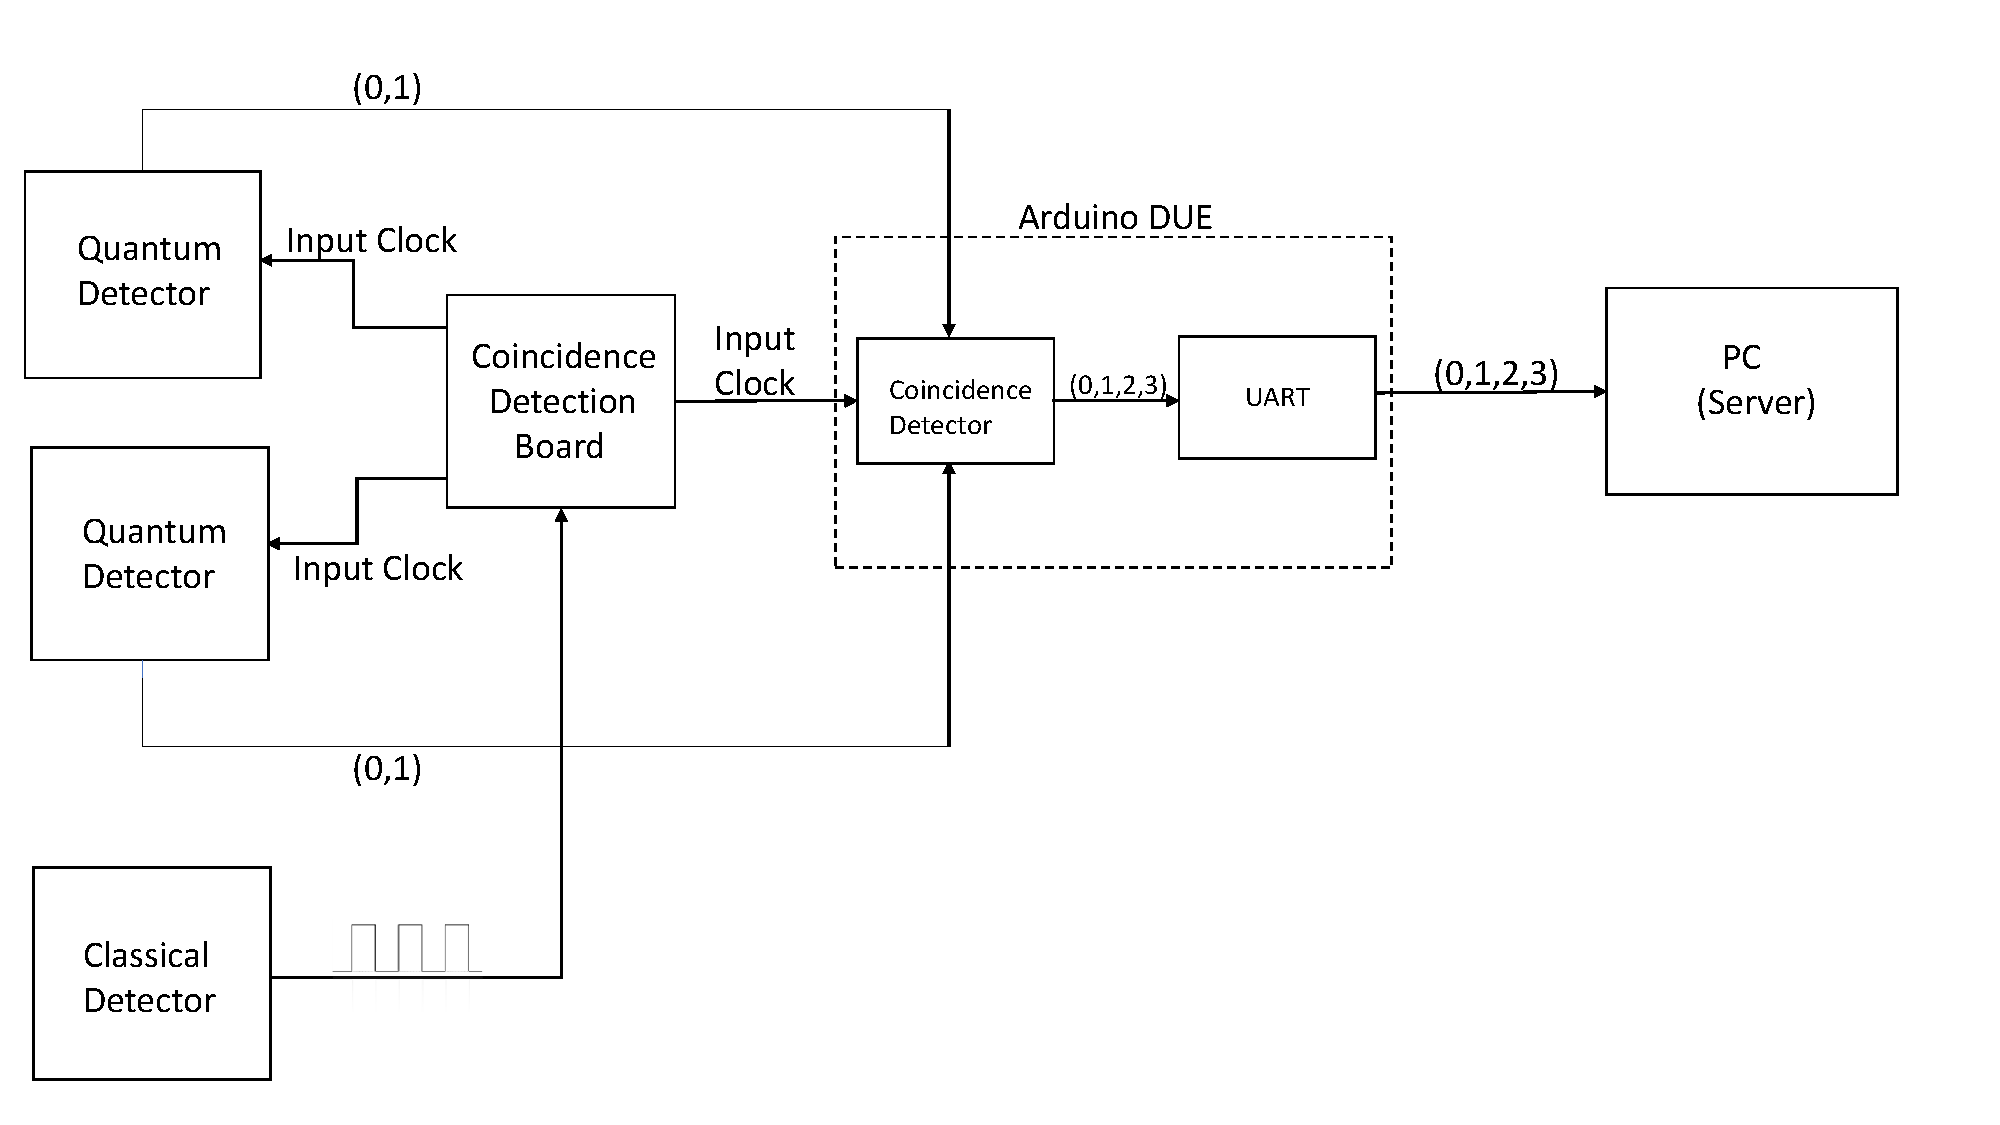
\includegraphics[width=1.1\linewidth]{./sdf/arduino_quantum_rx/figures/DiagramaGeralArduino.pdf}
		\caption{Block diagram of a arduino imlementation.}
		\label{fig:netxpto}
	\end{figure}
	
	
	\vspace{15px}
	\subsubsection{Clock signal}
	
	With purpose of processing the clock signal, it must be read by the digital Input pins of the arduino Due board. This type of reading doesnt require any signal conditioning witch means we can take direct measures from the clock into the arduino.The only note that is important to know is that max voltage the arduino due can take in the digital pins is 3.3V. When the arduino reads a "1" from the clock, it generates two separate 1kHz squares waves, they need to be sychronized with each other, which will be the trigger signal to the detectors.
	
	\vspace{15px}
	
   The clock signal can be seen in the next figure:
	
	\begin{figure}[H]
		\centering
		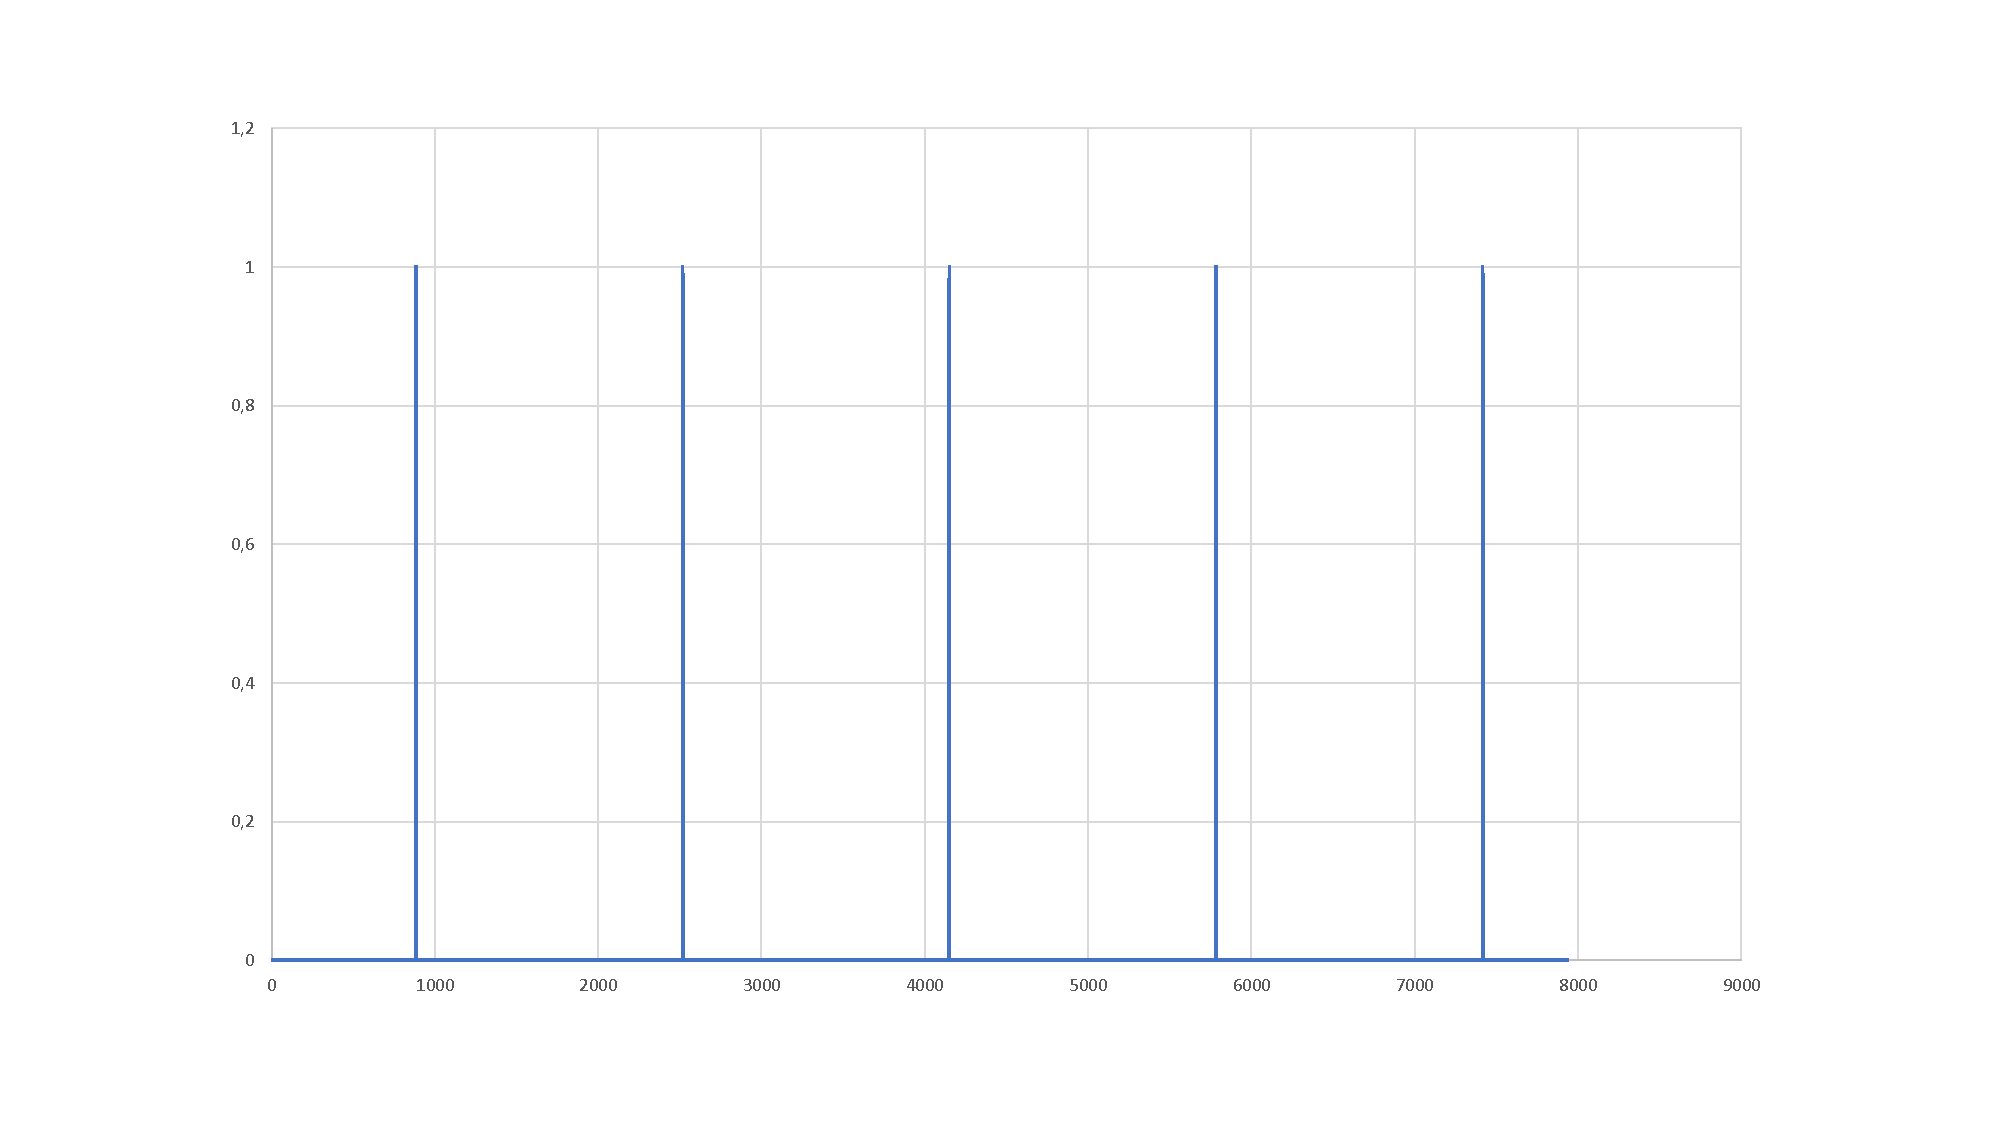
\includegraphics[width=1\linewidth]{./sdf/arduino_quantum_rx/figures/clockSignal2.pdf}
		\caption{Clock signal read.}
		\label{montage}
	\end{figure}

\subsubsection{SPD0 and SPD1 signals}

Since it is possible to control the TTL signal voltage that comes from the single photon detectors, we can measure them directly into the arduino board through the digital input pins. This signals are sychronized with the trigger signal that comes from the arduino. (Not yet implemented)
	
	
	\subsection{Open Issues}
	
	\clearpage
	\subsection{Visual Studio 2019 - Installation guide (Current version: 16.2.3)}
	
	\subsubsection{Step 1}
	
	The first thing to do is to download the bootstrapper file of this software through the following link: https://visualstudio.microsoft.com/pt-br/downloads/. As seen below in figure \ref{vstudio} one of three available versions can be choosen.
	
	\begin{figure}[H]
		\centering
		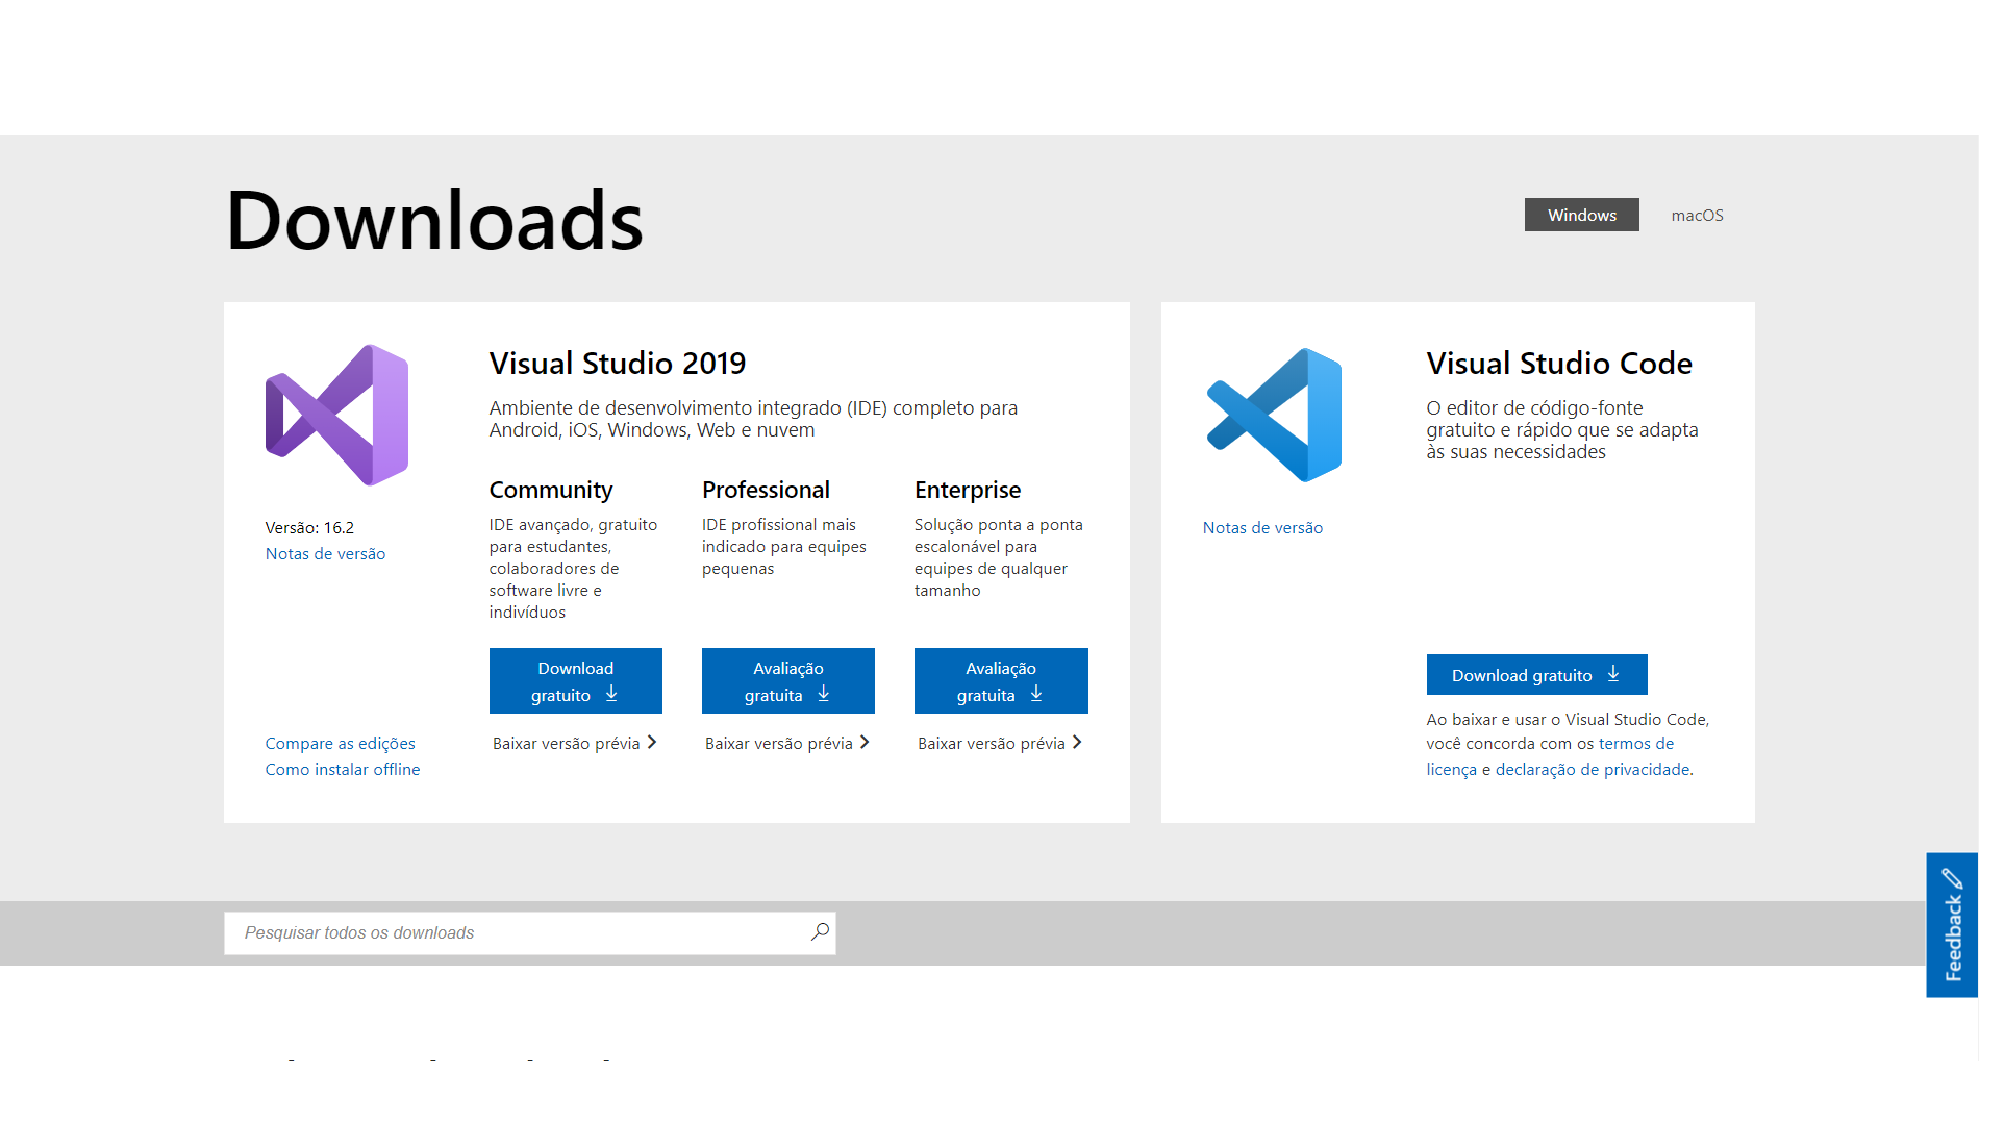
\includegraphics[width=1\linewidth]{./sdf/arduino_quantum_rx/figures/vsDownload.pdf}
		\caption{Download page of Visual Studio IDE software.}
		\label{vstudio}
	\end{figure}
	
	
	\subsubsection{Step 2}
	
	Execute the installer file, which you can use to customize your installation by selecting the feature sets or workloads, individual components, language packs and installation locations, as demonstrated in figure \ref{vstudioWorkloads}.
	
	
	
	\subsubsection{Step 3}
	
	The installation is quite simple and contains few steps for its execution, in case there is any doubt or question you can always get support from https://docs.microsoft.com/en-us/visualstudio/install/install-visual-studio?view=vs-2019.
	
	\begin{figure}[H]
		\centering
		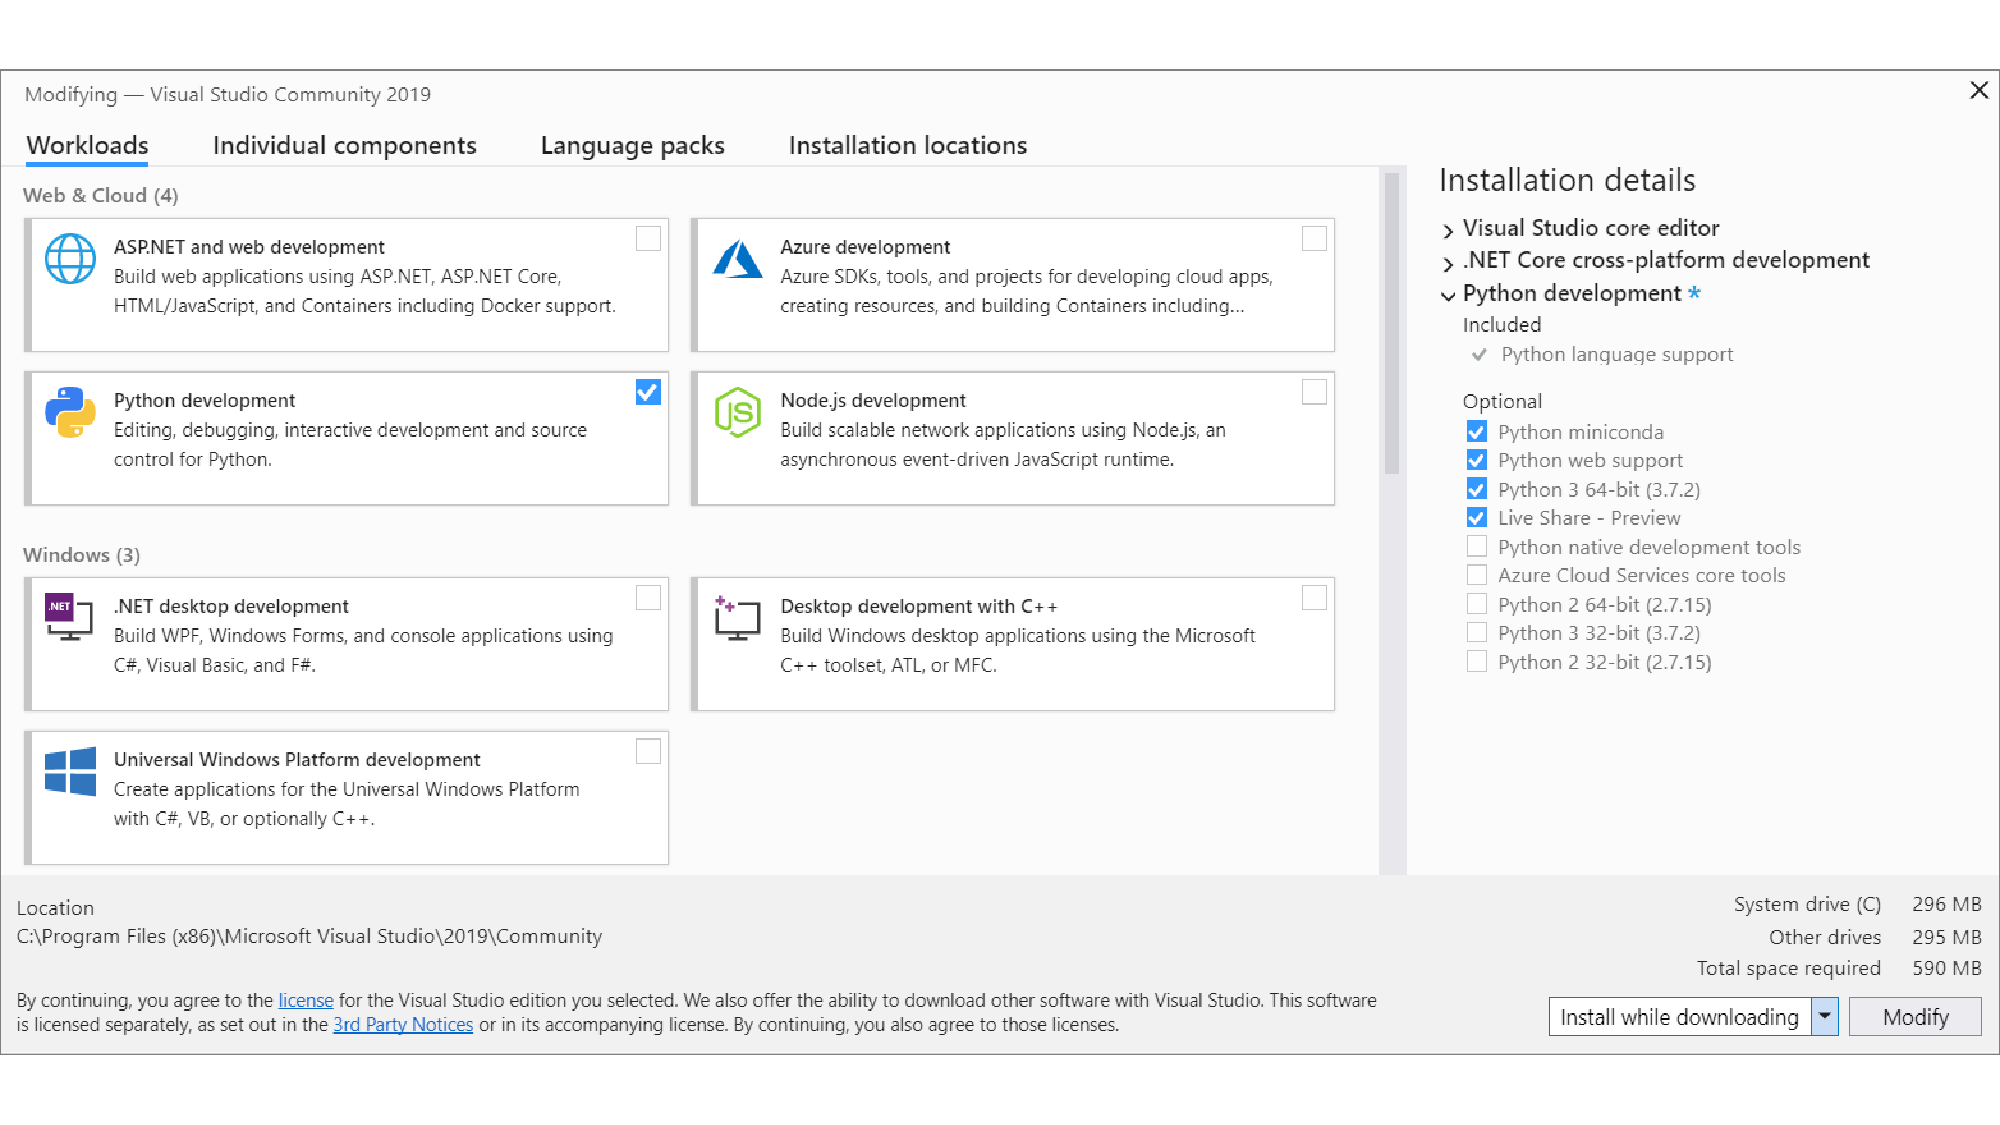
\includegraphics[width=1\linewidth]{./sdf/arduino_quantum_rx/figures/VSworkloads.pdf}
		\caption{Modifying - Visual Studio 2019.}
		\label{vstudioWorkloads}
	\end{figure}
	
	\subsection{Arduino IDE - Installation guide (Current version: 1.8.9) for Windows machines}
	
	\subsubsection{Step 1}
	
	Download the latest version of Arduino desktop IDE installer file from https://www.arduino.cc/en/main/software.
	
	\begin{figure}[H]
		\centering
		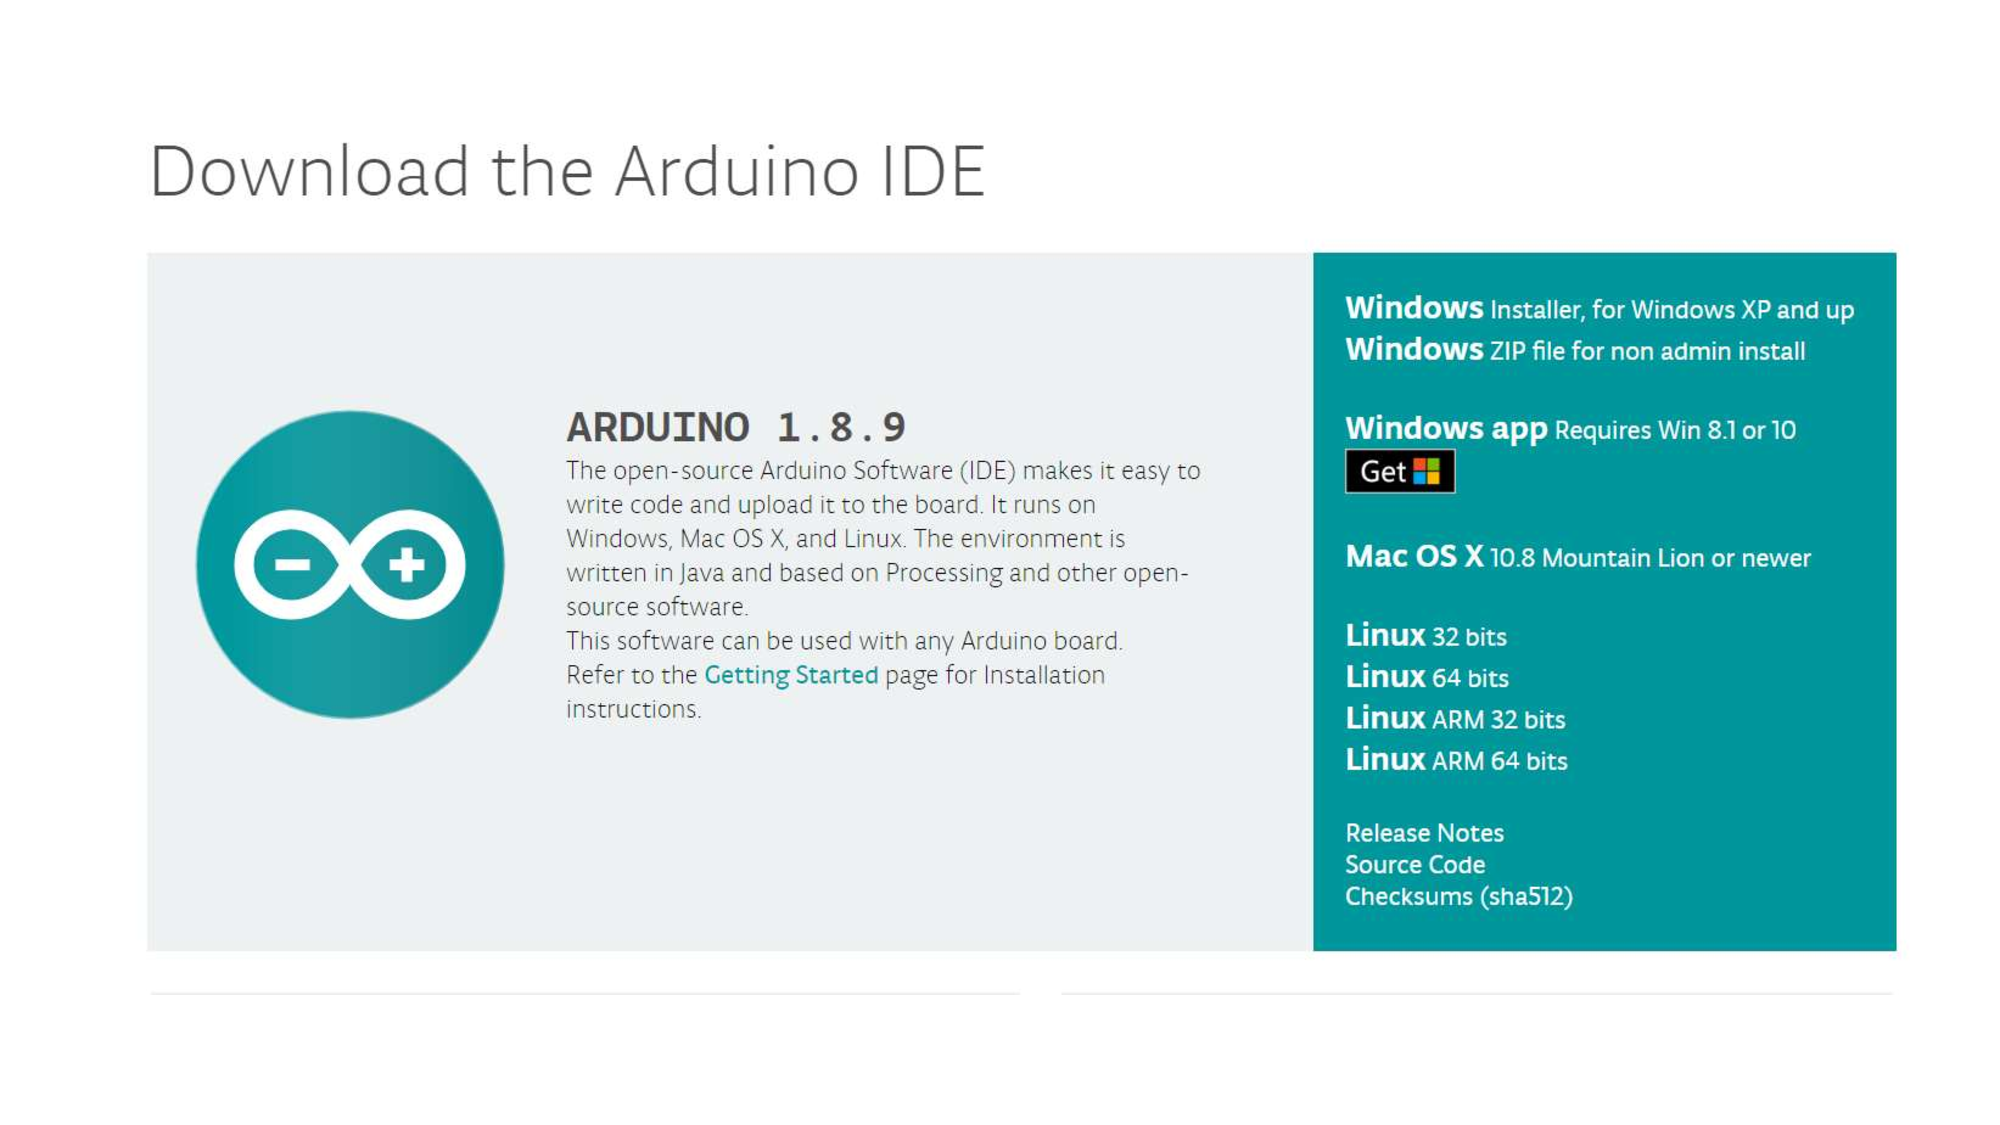
\includegraphics[width=0.86\linewidth]{./sdf/arduino_quantum_rx/figures/arduinoDownload.pdf}
		\caption{Download Arduino IDE software.}
		\label{arduinoDownload}
	\end{figure}
	
	
	\subsubsection{Step 2}
	
	When the download finishes, proceed with the installation and allow the driver installation process when you get a warning from the operating system. Follow the help guide present in https://www.arduino.cc/en/Guide/Windows.
	
	\subsubsection{Step 3}
	
	Proceed with the board specific instructions by going to https://www.arduino.cc/en/Guide/HomePage and selecting the respective board from the list provided, for this specific case we are considering the Arduino Due and so you can use the following link: https://www.arduino.cc/en/Guide/ArduinoDue.
	
	\begin{figure}[H]
		\centering
		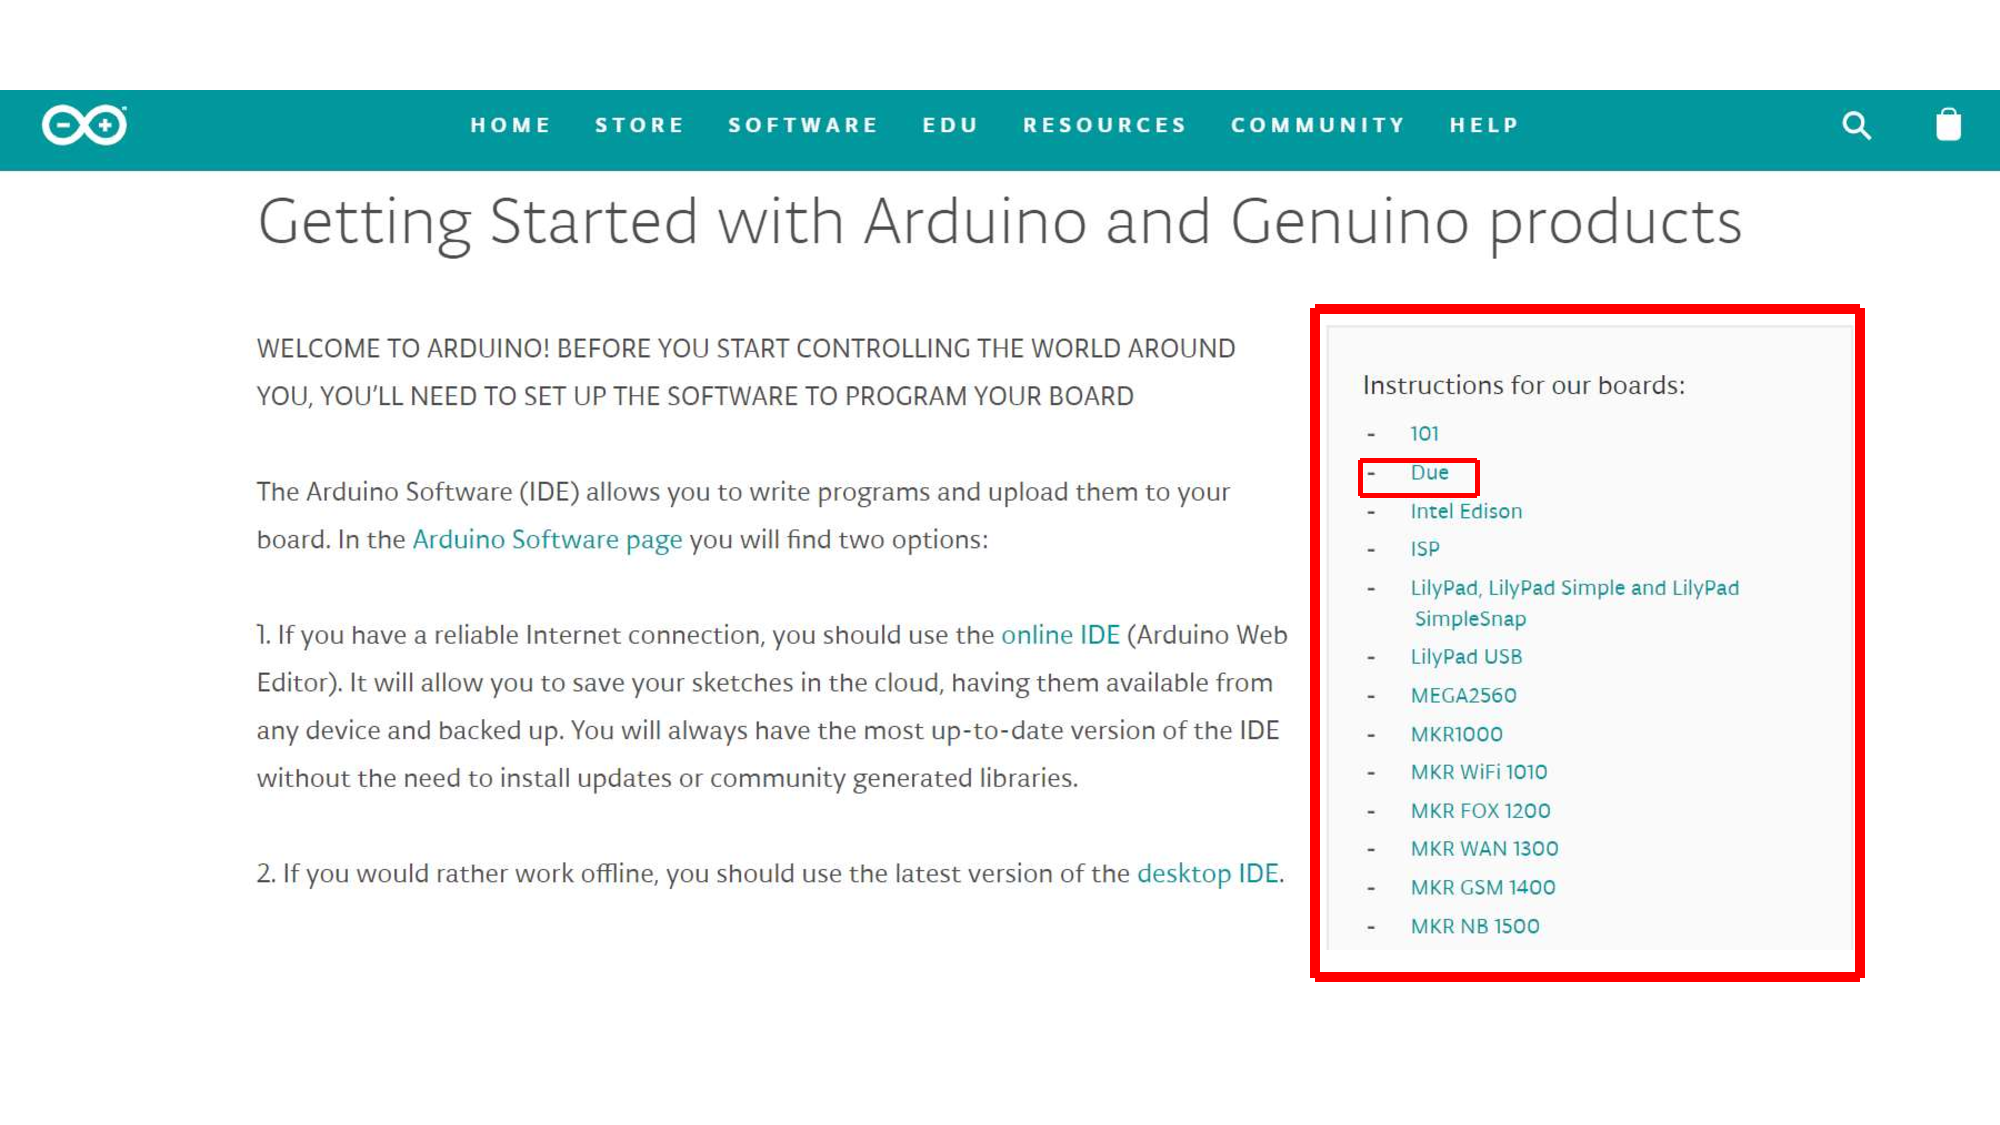
\includegraphics[width=1\linewidth]{./sdf/arduino_quantum_rx/figures/arduinoBoards.pdf}
		\caption{Select instructions for you specific board, in this case, the Arduino Due.}
		\label{arduinoDownload}
	\end{figure}
	
	\subsection{Visual Micro - Installation and Setup guide}
	Visual Micro is a plugin for Microsoft Visual Studio that helps you creating Arduino compatible cross-platform programs for hundreds of different Arduino compatible micro-controllers. Visual Micro supports projects that contain one or more .ino code files and standard c++ cource code files, just like the Arduino IDE.
	
	
	\subsubsection{Step 1}
	Download Visual Micro from here https://www.visualmicro.com/page/Arduino-Visual-Studio-Downloads.aspx or it can also be installed and uninstalled from inside the IDE, by opening Visual Studio and clicking "Extensions>Manage Extensions>Online>Arduino IDE for Visual Studio".
	
	\subsubsection{Step 2}
	If Visual Studio/Atmel Studio is running, then close it.
	
	\subsubsection{Step 3}
	Install Visual Micro by doubleclicking on the "vsix" icon of the downloaded file or in the case you are installing it from within the Visual Studio IDE it will start automatically.
	
	\subsubsection{Step 4}
	
	The first time, after you have installed Arduino for Visual Micro, the Configuration Manager will pop up where you can configure your system. Visual Micro must know the version and installation path of the Arduino IDE software that you have installed in your computer.
	
	\begin{figure}[H]
		\centering
		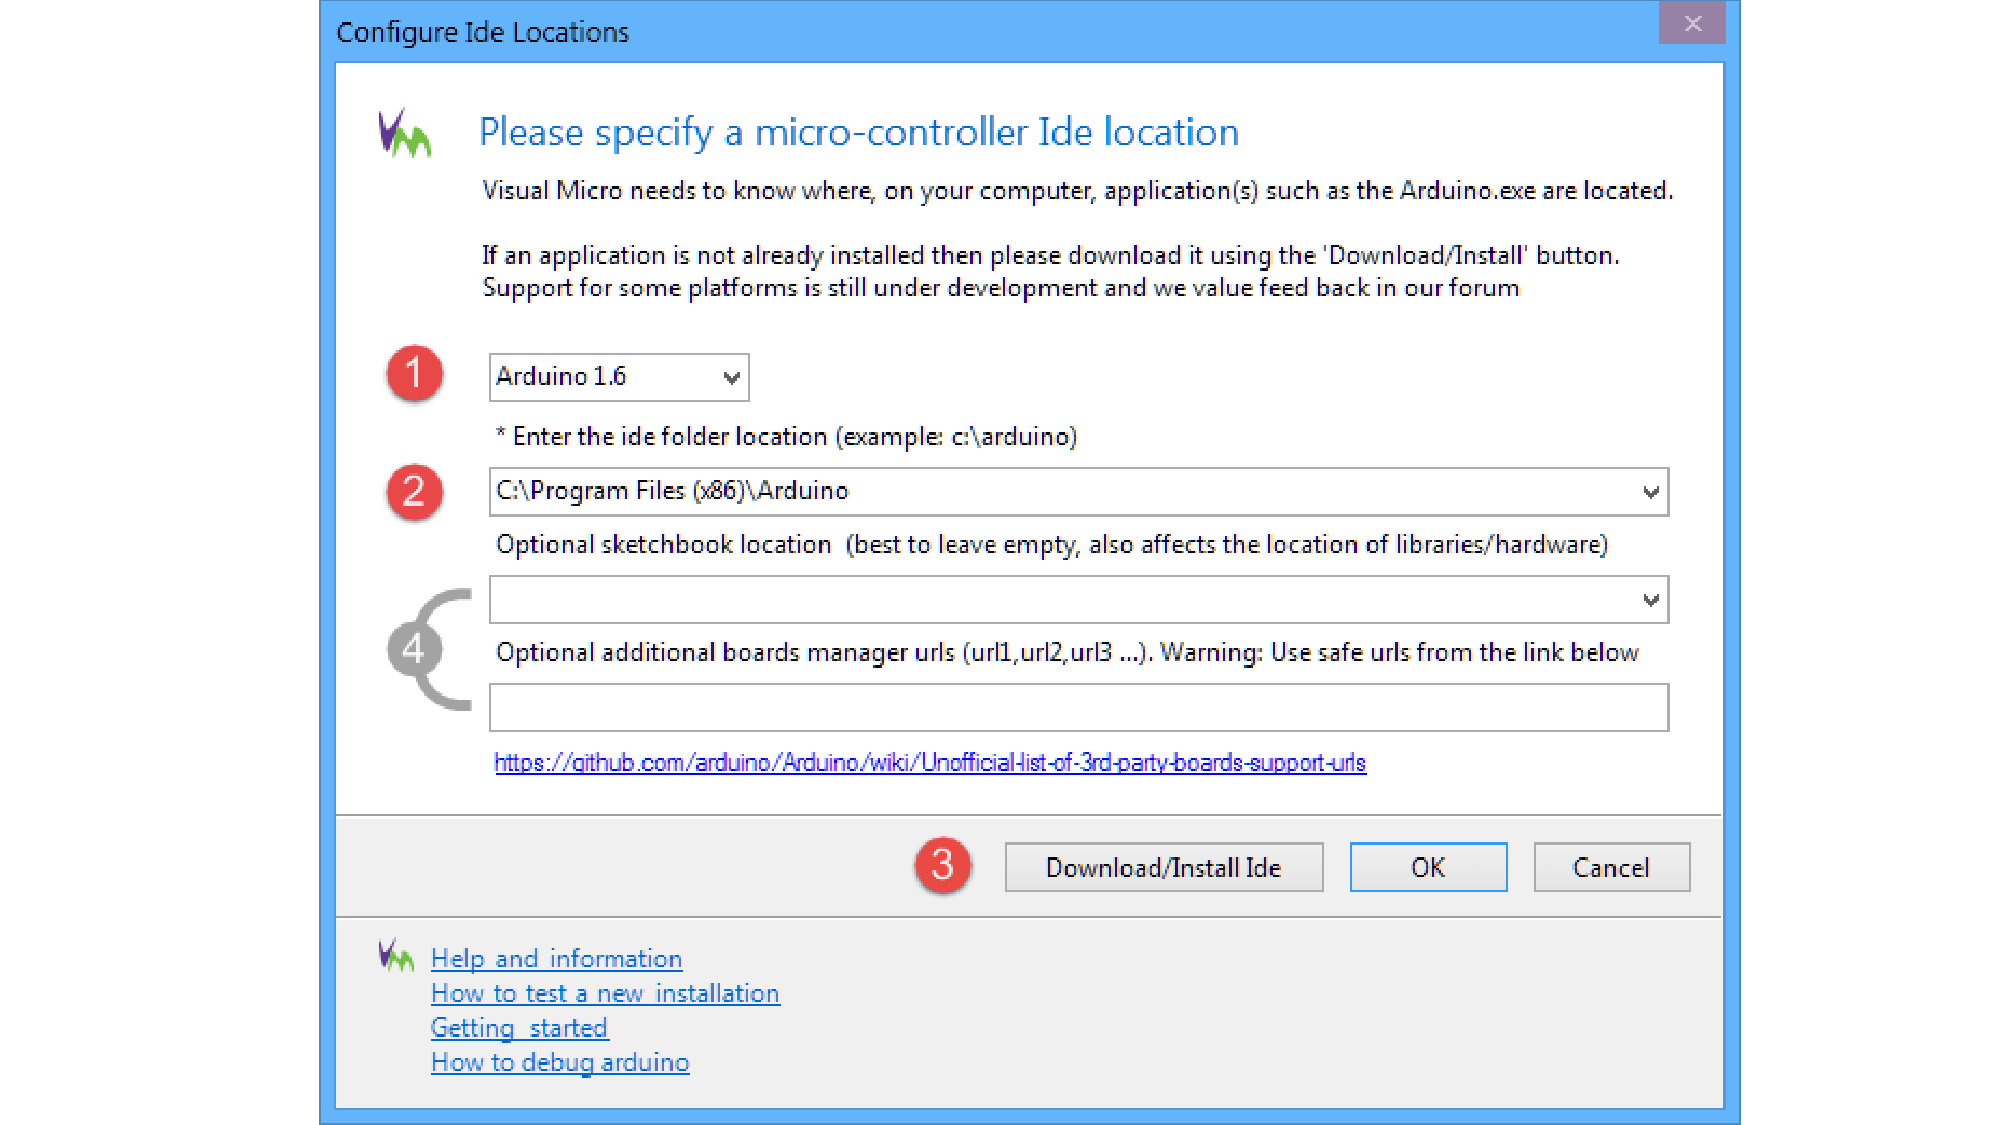
\includegraphics[width=1\linewidth]{./sdf/arduino_quantum_rx/figures/configureIDE.pdf}
		\caption{Configure IDE locations.}
		\label{configureIDE}
	\end{figure}
	
	\subsubsection{Step 4}
	If you work with different boards that required different IDEs, or if you have multiple versions of the Arduino IDE installed, then repeat the steps above for each IDE. It is possible to switch between configurations with the toolbar presented below in figure \ref{}.
	
	\begin{figure}[H]
		\centering
		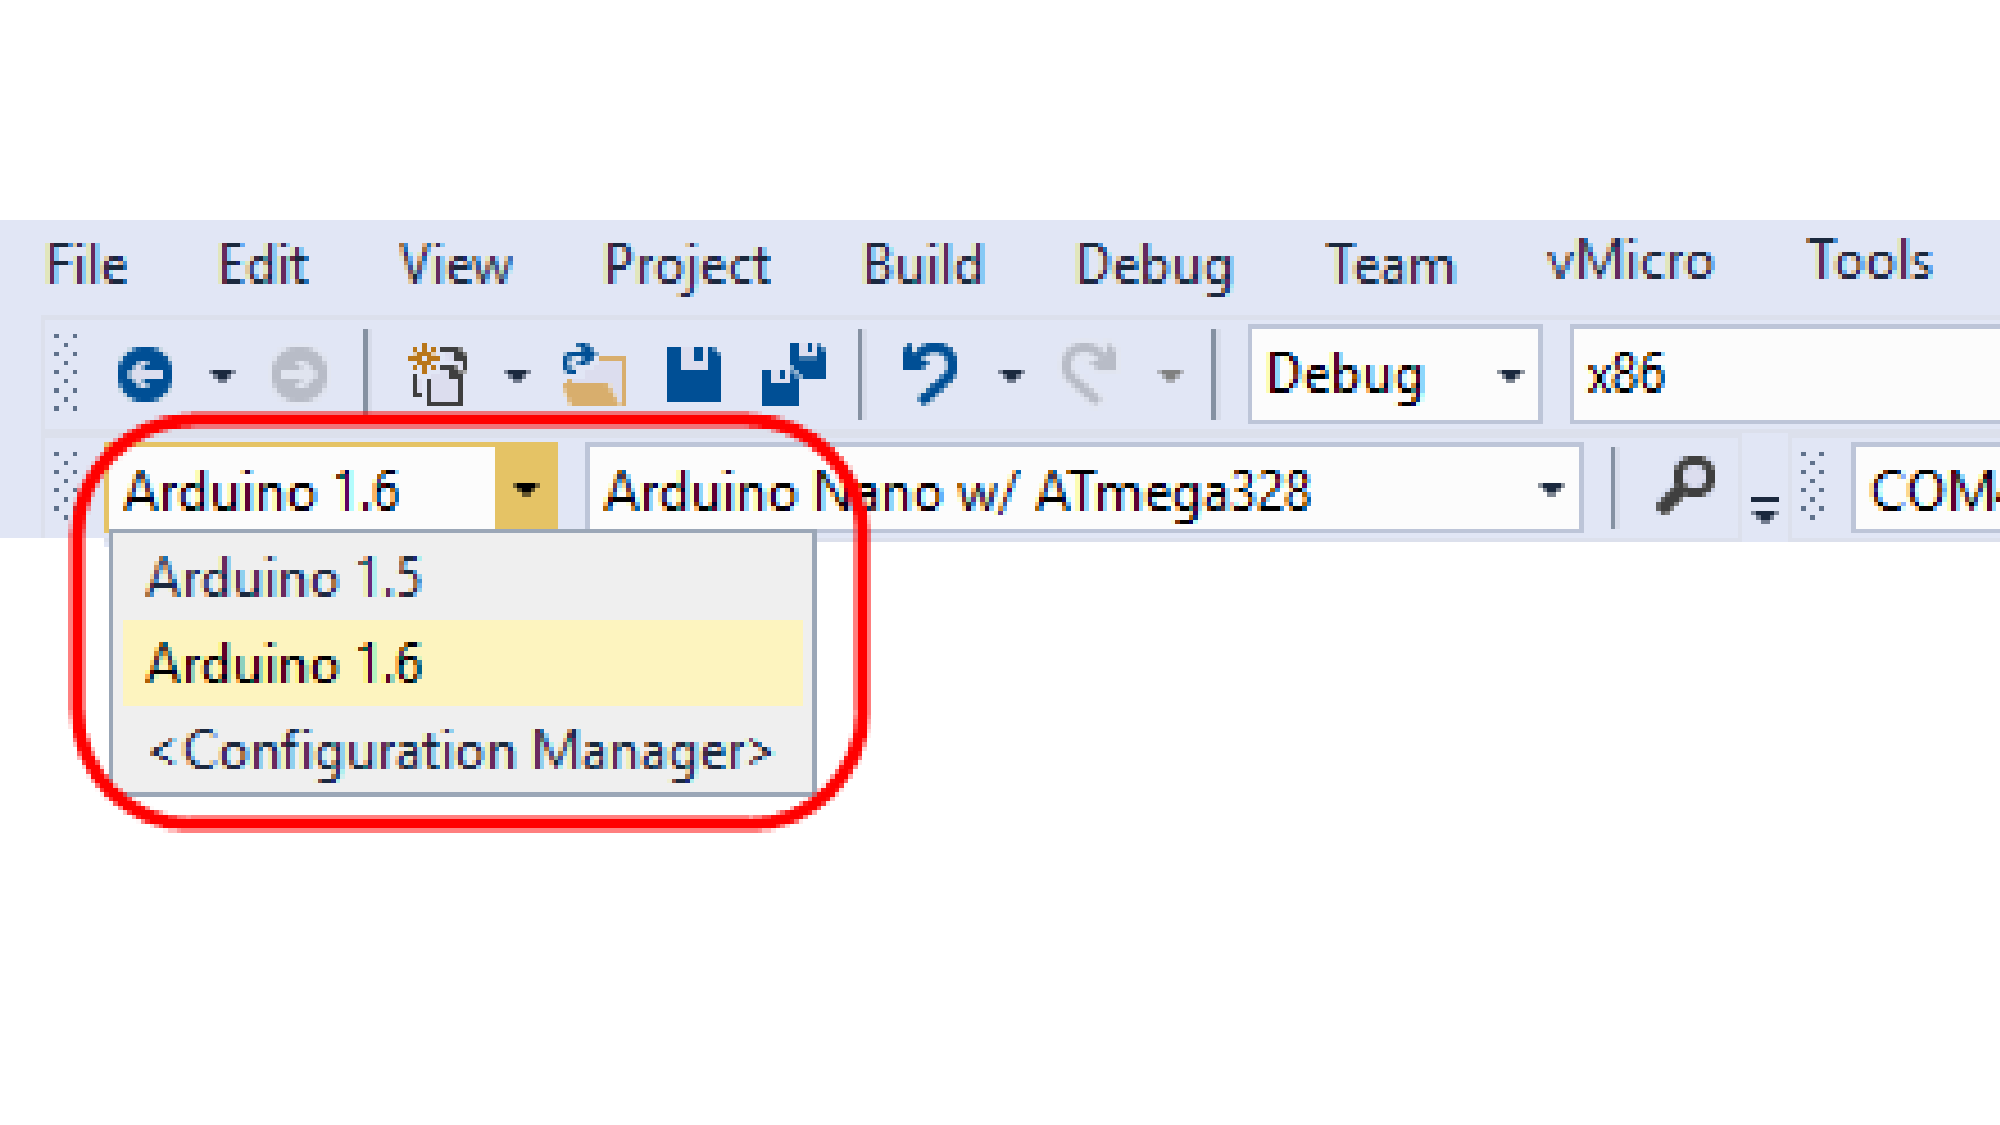
\includegraphics[width=0.7\linewidth]{./sdf/arduino_quantum_rx/figures/multipleIDEversions.pdf}
		\caption{Support for Multiple Versions of the Arduino Softwares.}
		\label{multipleIDEversions}
	\end{figure}
	
	
	\subsubsection{Step 5}
	
	In order to select the board model use the Visual Micro "Micro Boards" toolbar for that purpose, presented below. If the Visual Micro toolbar is missing, then you can show it by right clicking on an empty space in the toolbar area and checking "Micro Boards".
	
	
	\begin{figure}[H]
		\centering
		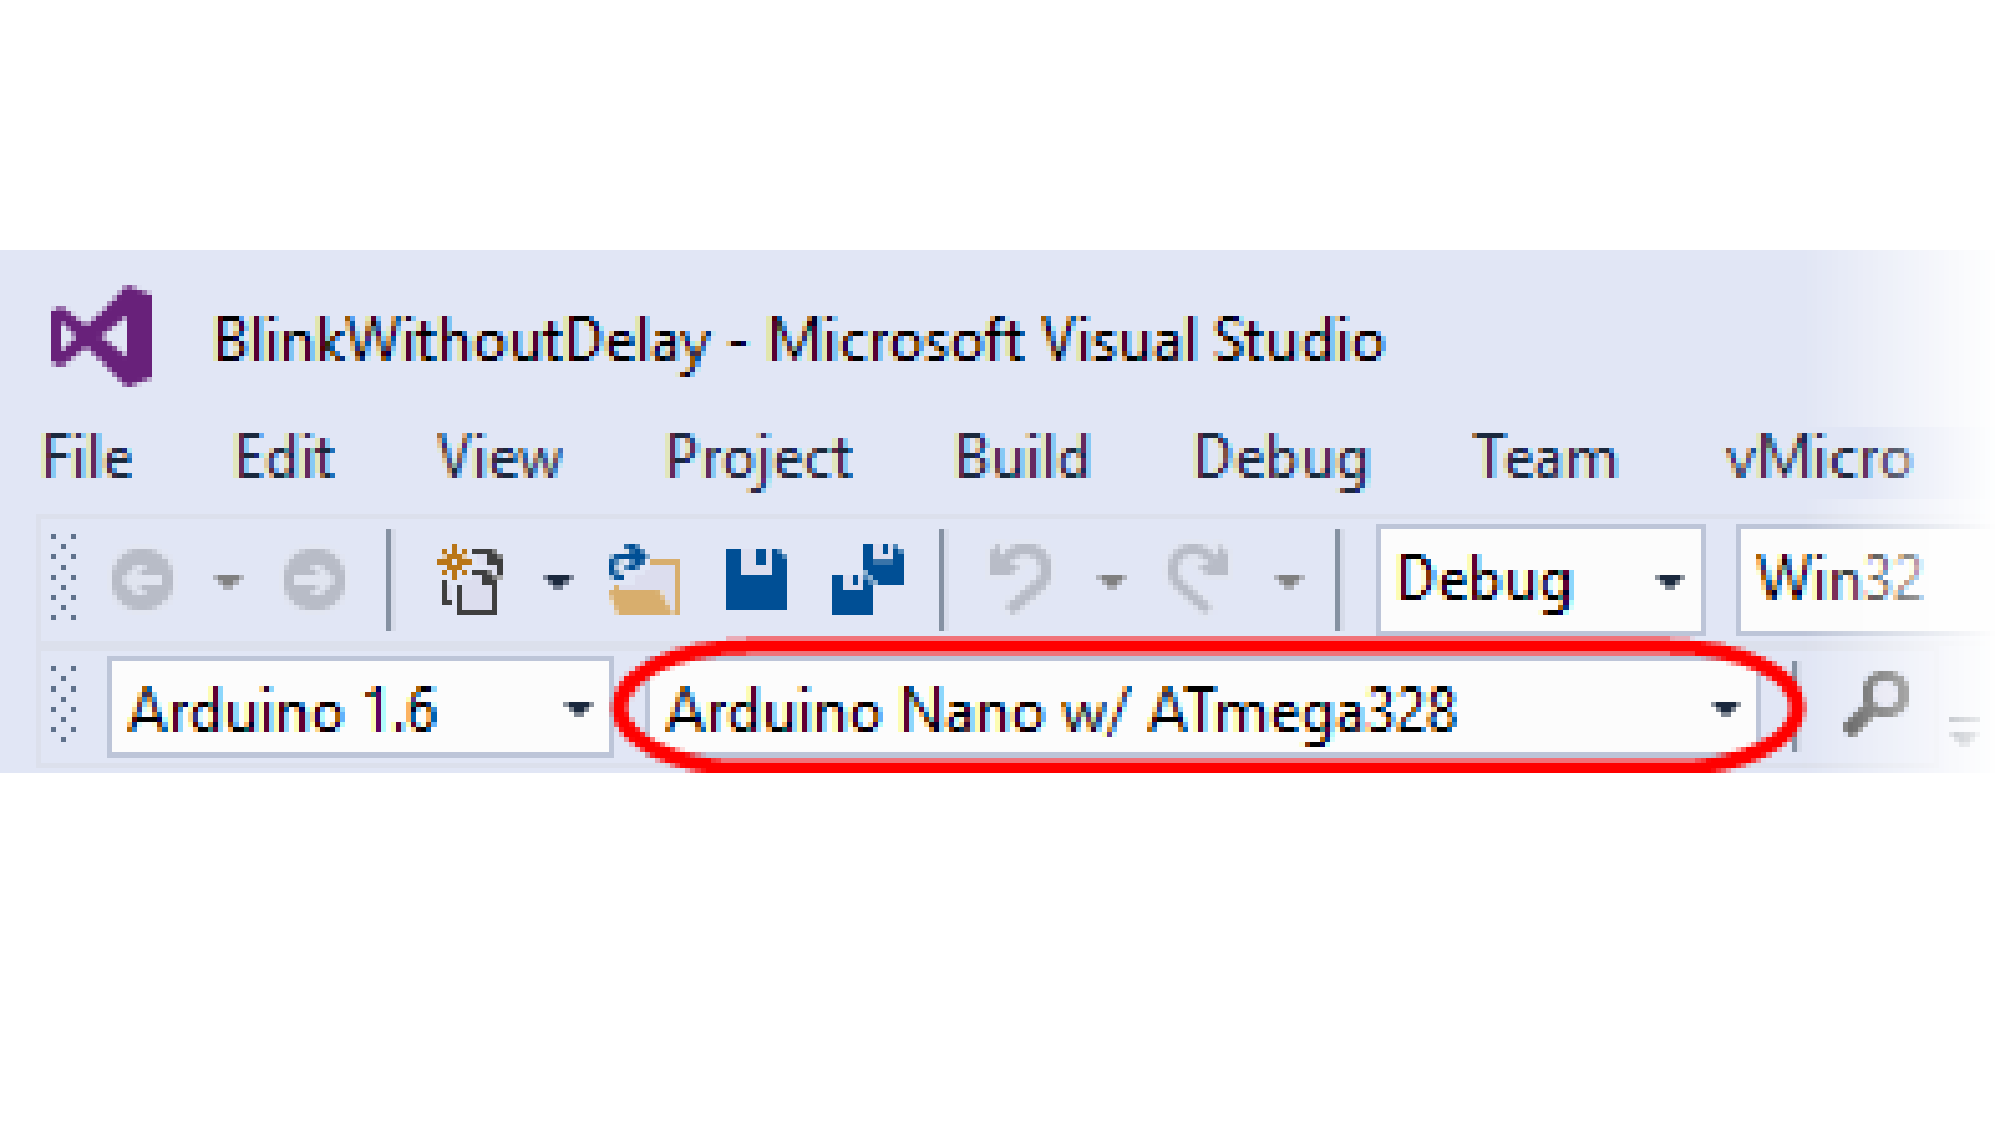
\includegraphics[width=0.7\linewidth]{./sdf/arduino_quantum_rx/figures/boardSelect.pdf}
		\caption{Selecting the Board Model.}
		\label{boardSelect}
	\end{figure}
	
	\subsubsection{Step 6}
	
	Connect your Arduino board to your PC using a USB cable. You must also tell your IDE which serial port to use and for that purpose use the Visual Micro Serial Communications toolbar shown below in figure \ref{selectSerial}. If the Visual Micro Serial Communications toolbar is missing, then you can show it by right clicking in the toolbar area and checking "Micro Serial Communications".
	
	\begin{figure}[H]
		\centering
		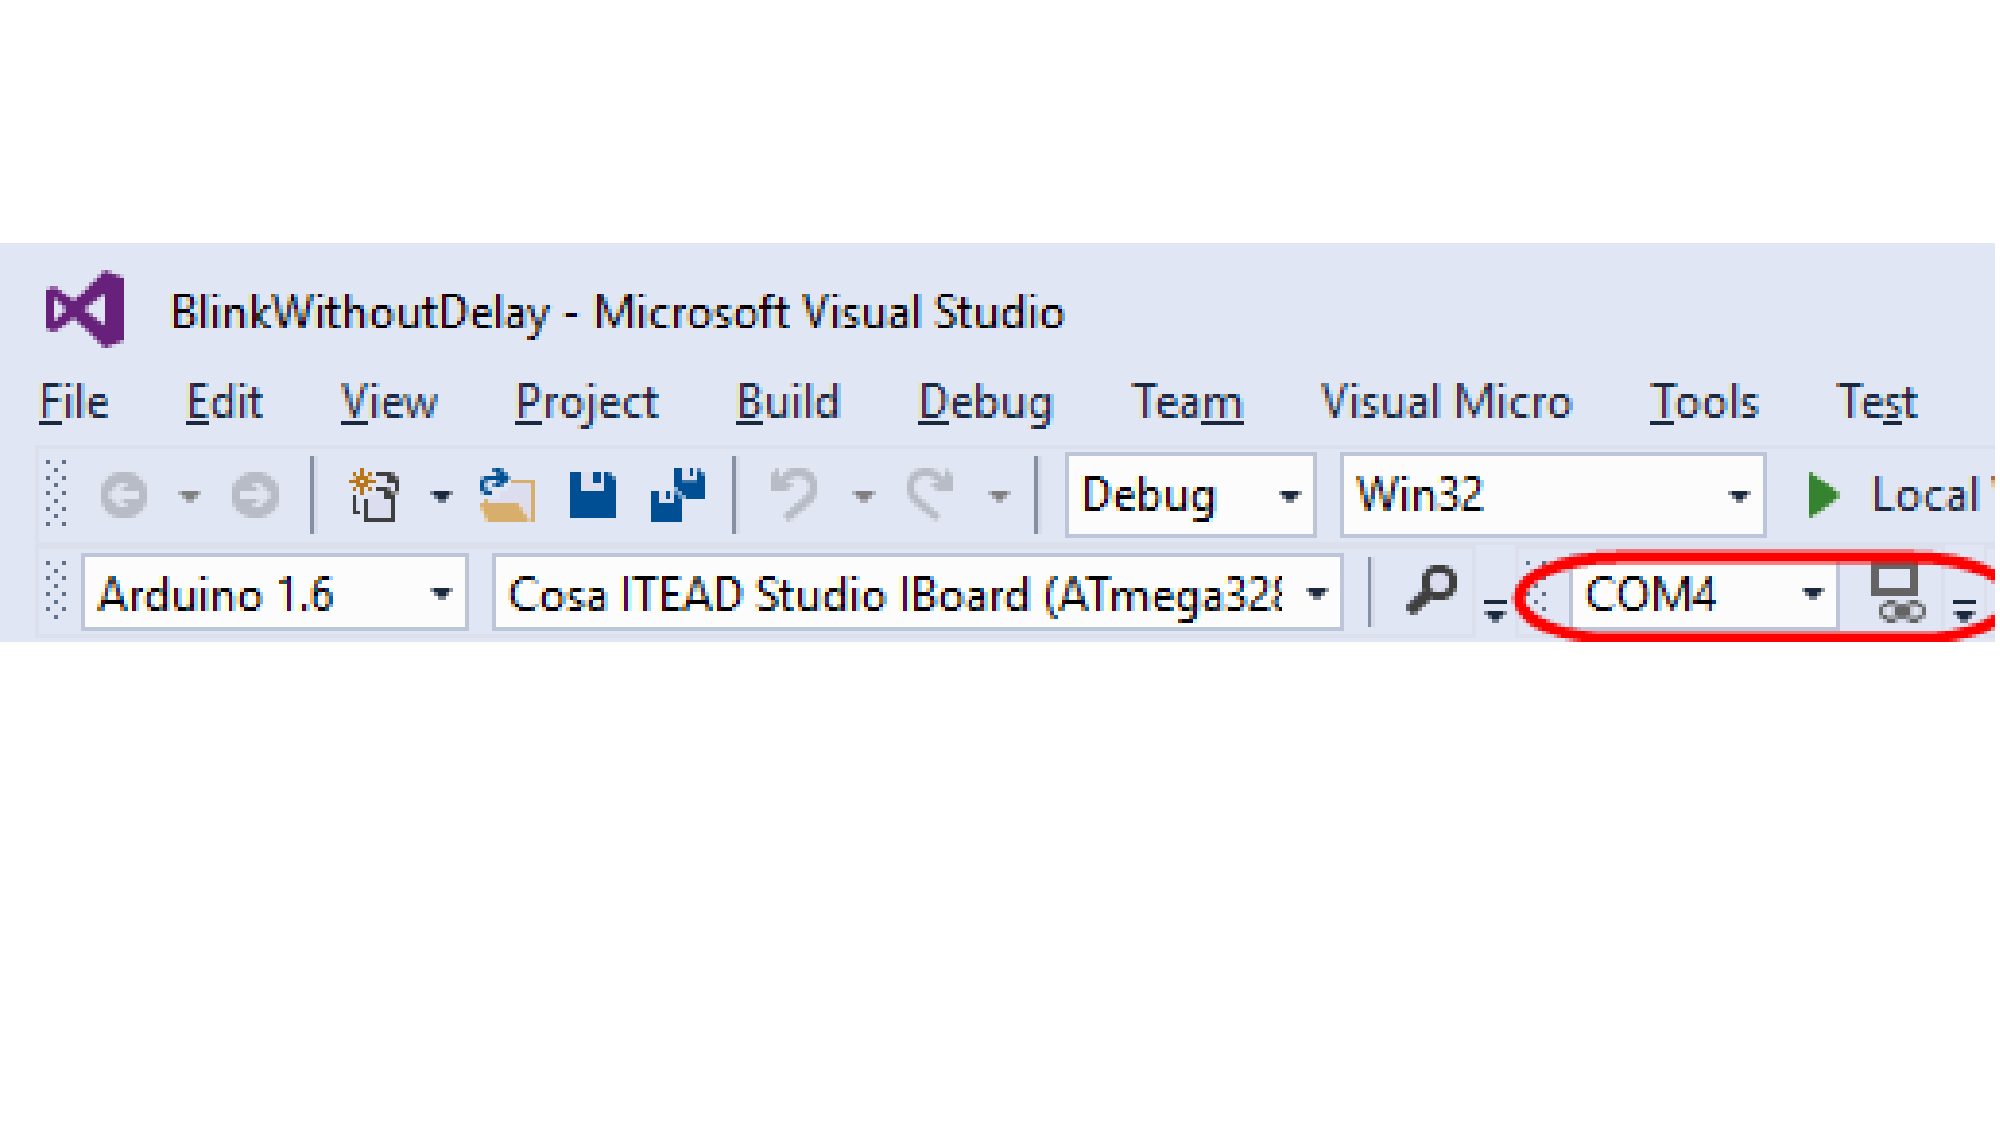
\includegraphics[width=0.7\linewidth]{./sdf/arduino_quantum_rx/figures/selectSerial.pdf}
		\caption{Setting up your Serial Port.}
		\label{selectSerial}
	\end{figure}
	
	\subsubsection{Step 7}
	At the end of these steps, you will be ready to write, compile, debug, and upload your Arduino sketches. In case of doubts consult the following link: https://www.visualmicro.com/page/User-Guide.aspx?doc=index.
	
	% bibliographic references for the section ----------------------------
	\clearpage
	\printbibliography[heading=subbibliography]
\end{refsection}
\addcontentsline{toc}{subsection}{Bibliography}
\cleardoublepage
% ---------------------------------------------------------------------
